% Included from both -slides and -handout versions.
\documentclass[pdftex]{beamer} % used to trigger beamer mode in Emacs,
                               % normally commented out.
\usetheme{metropolis}

\usepackage[english]{babel}
\usepackage[latin1]{inputenc}
\usepackage{graphicx}
\usepackage{times}
\usepackage[T1]{fontenc}
\usepackage{fancyvrb}
\usepackage{listings}
\begin{document}
\lstset{language=C, escapeinside={(*@}{@*)}, numbers=left,
  basicstyle=\tiny, showspaces=false, showtabs=false}

\title{Introduction to Operating Systems}
\subtitle{Through tracing, analysis, and experimentation}
%\institute{University of Cambridge}
\author{George V. Neville-Neil \& Dr Robert N. M. Watson}
\date{3 August 2016}

\begin{frame}
  \titlepage
\end{frame}

\begin{frame}[fragile]
  \frametitle{Day Plan}
  \begin{tabular*}{1.0\linewidth}{l|l}
    Time & Topic \\
    \hline
    09:15-09:45 & \textbf{Processes} \\
    09:45-10:00 & Break \\
    10:00-12:00 & Locking \\
    12:00-13:00 & Lunch \\
    13:00-14:15 & Virtual Memory \\
    14:15-14:30 & Break \\
    14:30-16:30 & Lab 2 \\
    16:30-17:00 & Lab 2 Review
  \end{tabular*}
\end{frame}


\begin{frame}
  \frametitle{Review}
  \begin{itemize}
  \item History
  \item UNIX Like Systems
  \item Debugging and Tracing
  \end{itemize}
\end{frame}

\section{Processes}
\label{sec:processes}

\begin{frame}
  \frametitle{Review: What is an Operating System?}
  \begin{itemize}
  \item Provider of useful abstractions
  \item Generic interface to varied hardware resources
  \item Controller of resources
  \item Provider of basic security
  \end{itemize}
\end{frame}

\begin{frame}
  \frametitle{The process model}
  \begin{enumerate}
    \item The process model and its evolution
    \item Where do programs come from?
    \item Traps and system calls
    \item An introduction to virtual memory
  \end{enumerate}
\end{frame}

\begin{frame}
  \frametitle{Before Processes and Virtual Memory}
  \begin{itemize}
  \item All code in a single address space
  \item No memory protection
  \item Each program must cooperate with all others
  \item Core wars
  \end{itemize}
\end{frame}

\begin{frame}
  \frametitle{What is a process?}
  \begin{itemize}
  \item Container for code
  \item Protective shell between competing programs
  \item \emph{The} defining abstraction on which all modern computing rests
  \end{itemize}
\end{frame}

\begin{frame}
  \frametitle{Process Contents}
\begin{columns}[t]
    \begin{column}{5cm}
      \begin{itemize}
      \item Open Files
      \item Process Statistics
      \item Resource Limits
      \item Signal Actions
      \item Process Identifier (PID)
      \item Lists of related processes
      \item Many Locks and Mutexes
      \end{itemize}
    \end{column}
    \begin{column}{5cm}
      \begin{itemize}
      \item Address Space
      \item Alarms and Timers
      \item Resource Usage
      \item Threads
      \item Debugging 
      \item Security
      \item $112$ total fields
      \end{itemize}
    \end{column}
  \end{columns}
\end{frame}

\begin{frame}
  \frametitle{The UNIX process life cycle}

  \begin{columns}[T]
    \column{0.5\textwidth}
      \vspace{0.5cm}
      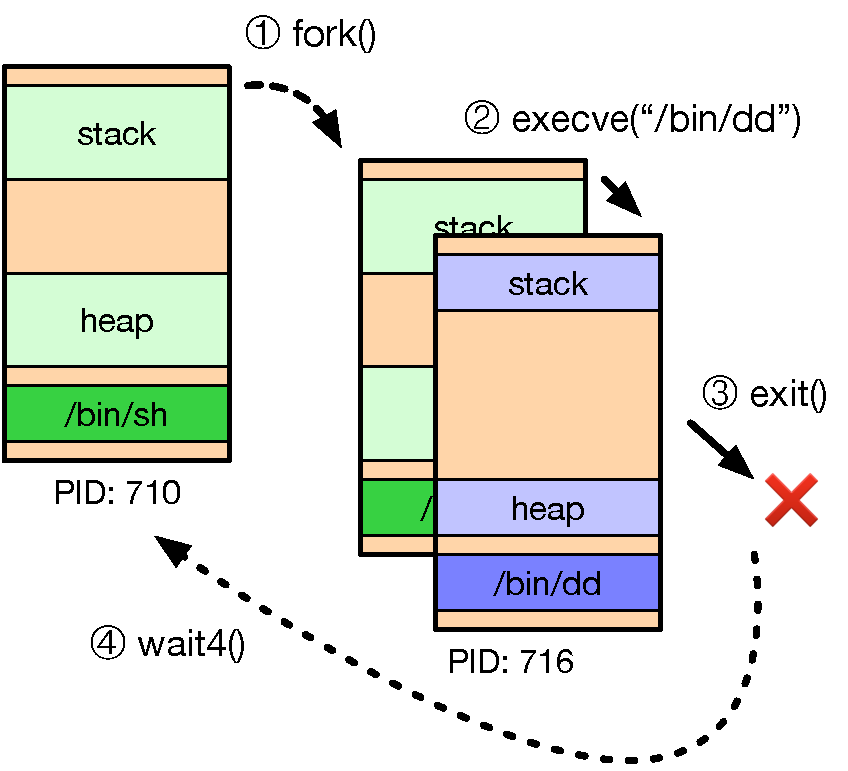
\includegraphics[width=\textwidth]{../../figures/process-life-cycle.pdf}

    \column{0.5\textwidth}
    \begin{itemize}

      \pause

      \item \texttt{fork()}
      \begin{itemize}
	\item Child inherits address space and other properties
	\item Program prepares process for new binary (e.g., \texttt{stdio})
	\item Copy-on-Write (COW)
      \end{itemize}

      \pause

      \item \texttt{execve()}
      \begin{itemize}
	\item Kernel replaces address space, loads new binary, starts execution
      \end{itemize}

      \pause

      \item \texttt{exit()}
      \begin{itemize}
	\item Process can terminate self (or be terminated)
      \end{itemize}

      \pause

      \item \texttt{wait4} (et al)
      \begin{itemize}
	\item Parent can await exit status
      \end{itemize}
    \end{itemize}
  \end{columns}
\end{frame}

\begin{frame}[fragile]
  \frametitle{Who is forking?}
\begin{lstlisting}
dtrace -n 'syscall::*fork:entry { @forks[execname] = count();}'
dtrace: description 'syscall::*fork:entry ' matched 8 probes
^C
  csh                                                            7031
\end{lstlisting}
\end{frame}

\begin{frame}[fragile]
  \frametitle{Fork Discussion}
  \begin{itemize}
  \item Why do we use a wild card?
    \begin{itemize}
    \item \verb+syscall::*fork:entry+
    \end{itemize}
  \end{itemize}
\end{frame}

\begin{frame}
  \frametitle{Proc Provider}
  \begin{description}
  \item[exec] Program execution attempt
  \item[exec-failure] Program start failed
  \item[exec-success] Program successfully started
  \item[exit] Program terminated
  \item[signal-send] Send a signal
  \item[signal-clear] Cleared a signal
  \item[signal-discard] Signal ignored
  \end{description}
\end{frame}

\begin{frame}
  \frametitle{Scheduling}
  \begin{itemize}
  \item Control over CPU resources
  \item Which process or thread can run now?
  \end{itemize}
\end{frame}

\begin{frame}[fragile]
  \frametitle{The Scheduler}
  \begin{itemize}
  \item Decides which thread gets to run
  \item The \emph{thread} is the scheduable entity
  \item Chooses a processor/core
  \item Can be overridden by \verb+cpuset+
  \end{itemize}
\end{frame}

\begin{frame}
  \frametitle{Process States}
  \begin{description}
  \item[NEW] Being created
  \item[RUNNABLE] Can run
  \item[SLEEPING] Awaiting some event
  \item[STOPPED] Debugging
  \item[ZOMBIE] Process of dying
  \end{description}
\end{frame}

\begin{frame}
  \frametitle{Scheduling Classes}
  \begin{description}
  \item[ITHD] interrupt thread
  \item[REALTIME] real-time user
  \item[KERN] kernel threads
  \item[TIMESHARE] normal user programs
  \item[IDLE] run when nothing else does
  \end{description}
\end{frame}

\begin{frame}[fragile]
  \frametitle{Sched Provider}
  \begin{description}
  \item[on-cpu] Thread moves on core
  \item[off-cpu] Thread moves off core
  \item[remain-cpu] Thread remains on core
  \item[change-pri] Priority changed
  \item[fbt:kernel:cpu\_idle:entry] Thread went idle
  \end{description}
\end{frame}

\begin{frame}[fragile]
  \frametitle{Context Switching}
  \begin{itemize}
  \item Processes all believe they own the computer
  \item Context switching maintains this fiction
  \item Requires saving and restoring state
  \item Common measure of operating system performance
  \item \verb+cswstat.d+ measures overall context switching
  \end{itemize}
\end{frame}

\section{Mutual Exclusion and Locking}
\label{sec:locking}

\begin{frame}
  \frametitle{What is Locking, and why do we need it?}
  \begin{itemize}
  \item Protection of shared resources
  \item Prevent incorrect updates
  \item Required in OS kernels before multi-core systems
    \begin{itemize}
    \item Devices are a source of asynchronous events
    \end{itemize}
  \end{itemize}
\end{frame}

\begin{frame}
      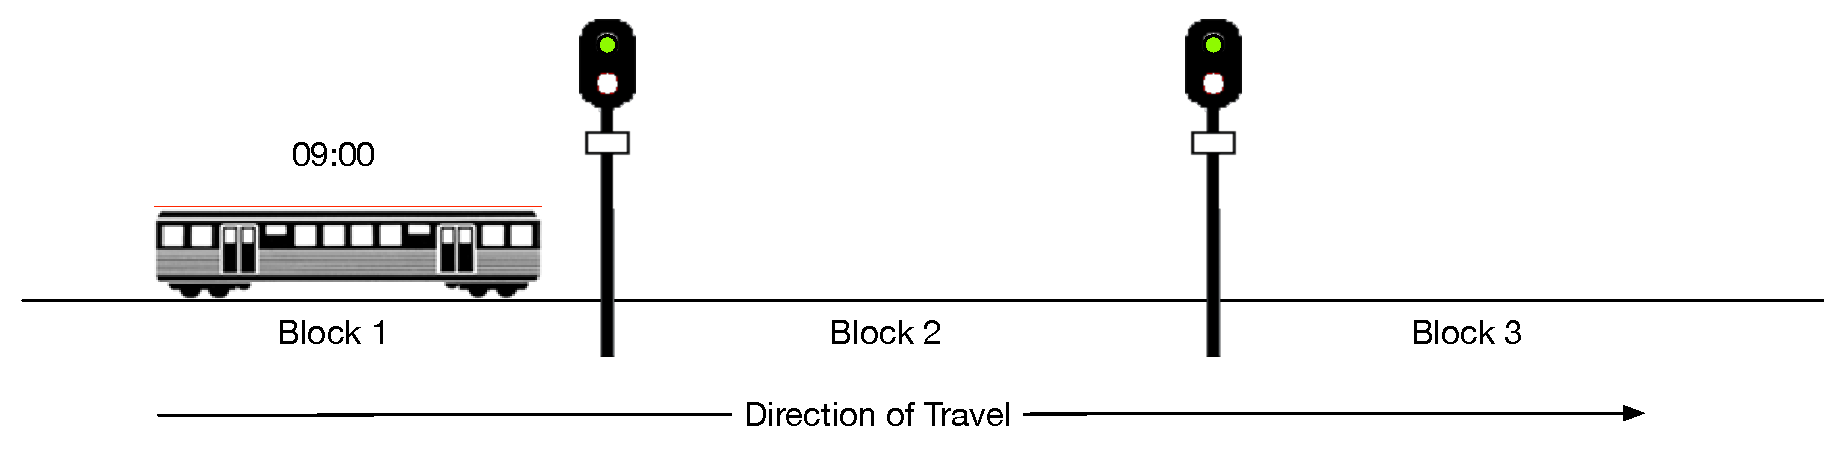
\includegraphics[width=\textwidth]{../../figures/block-signaling-1.pdf}
\end{frame}

\begin{frame}
      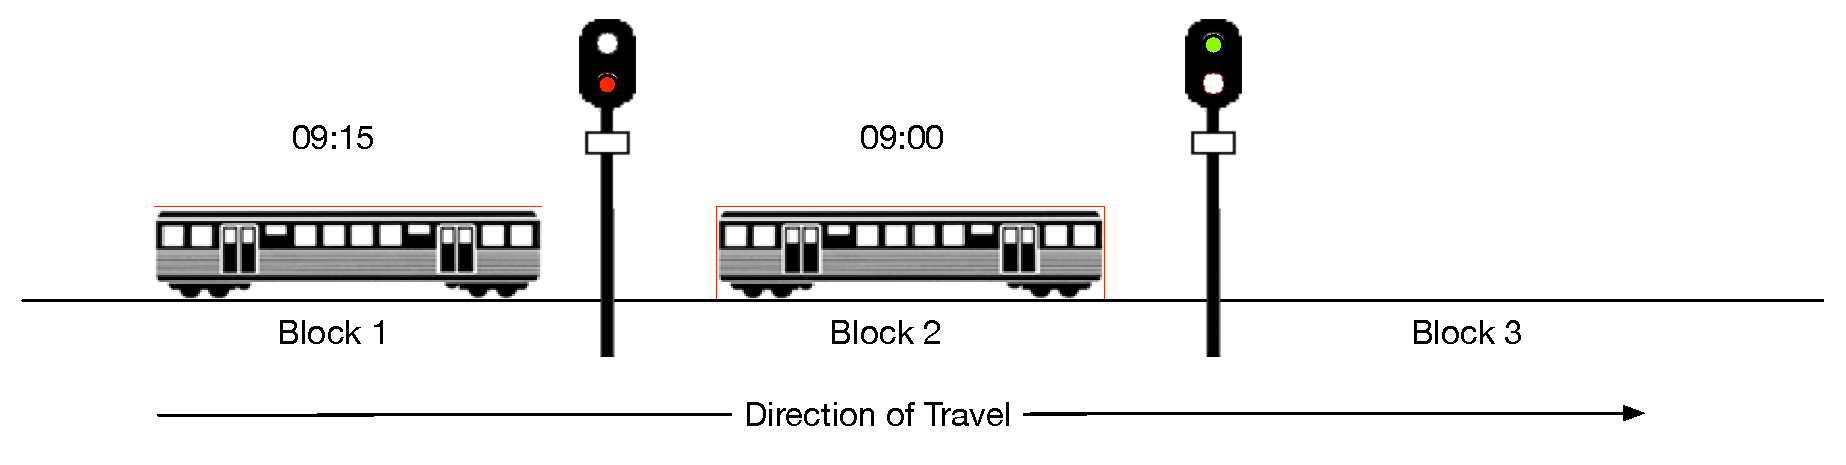
\includegraphics[width=\textwidth]{../../figures/block-signaling-2.pdf}
\end{frame}

\begin{frame}
      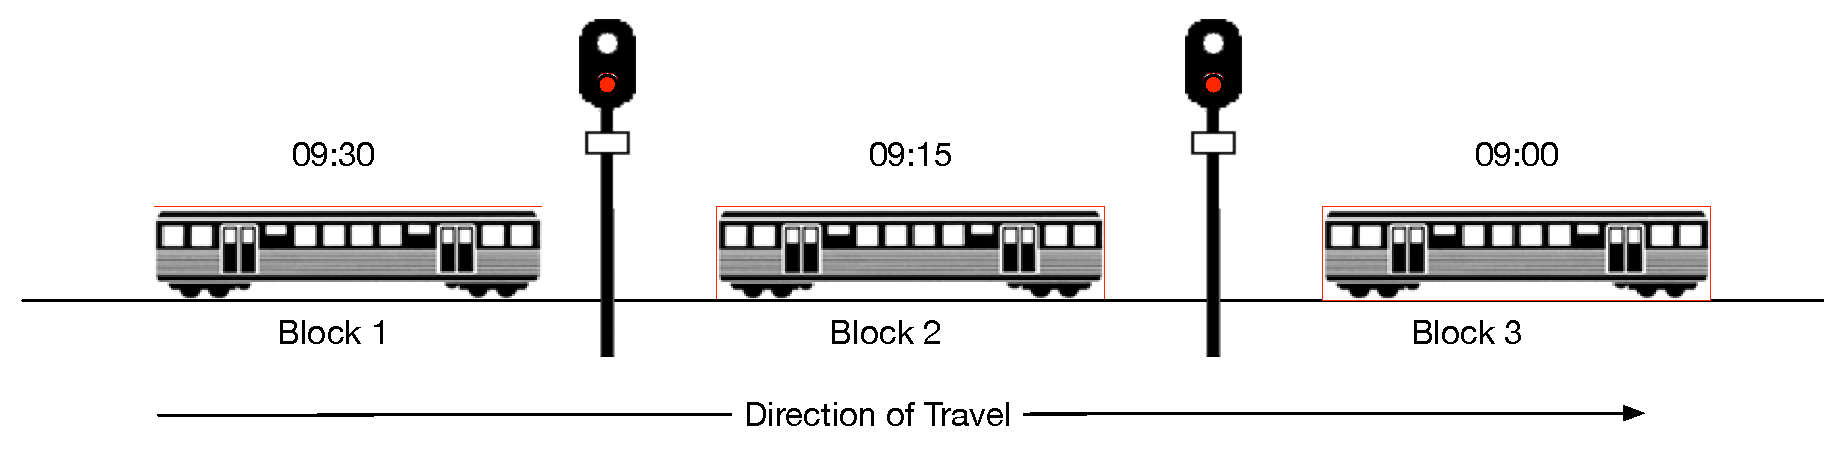
\includegraphics[width=\textwidth]{../../figures/block-signaling-3.pdf}
\end{frame}

\begin{frame}
  \frametitle{CPUs, Cores, Threads and Locking}
  \begin{itemize}
  \item Past the end of frequency scaling
  \item One CPU die has many cores
  \item The number of cores increases year on year
    \begin{itemize}
    \item ARMv8 has 48 cores per die, 96 cores per system
    \end{itemize}
  \item The kernel may now be the largest multi-threaded program in history.
  \end{itemize}
\end{frame}

\begin{frame}
  \frametitle{Locking Overview}
  \begin{itemize}
  \item Multiple hardware threads
  \item Protection for kernel shared state
    \begin{itemize}
    \item The kernel's lists and hash tables
    \end{itemize}
  \item Locking required for multi-core systems
  \end{itemize}
\end{frame}

\begin{frame}[fragile]
  \frametitle{What is locked in the kernel?}
  \begin{columns}[t]
    \begin{column}{5cm}
      \begin{itemize}
      \item Processes
      \item File Systems
      \item Name Cache
      \item Network Sockets
      \item Routing Tables
      \item Interface Lists
      \item Firewall Rules
      \end{itemize}
    \end{column}
    \begin{column}{5cm}
      \begin{itemize}
      \item Virtual Memory System
      \item All Device Drivers
      \item Timers and Callouts
      \item Terminals and Console
      \item Network Protocol Lists
      \item \emph{Any shared resource}
      \end{itemize}
    \end{column}
  \end{columns}
\end{frame}

\begin{frame}
  \frametitle{What is a lock?}
  \begin{itemize}
  \item A data stucture that seriealizes acess to a resource
  \end{itemize}
\end{frame}

\begin{frame}
  \frametitle{The Problems of Locking }
  \begin{description}
  \item[Deadlock] System unable to make forward progress
  \item[Starvation] One part of the system always gets the lock
  \end{description}
\end{frame}

\begin{frame}
\centering
      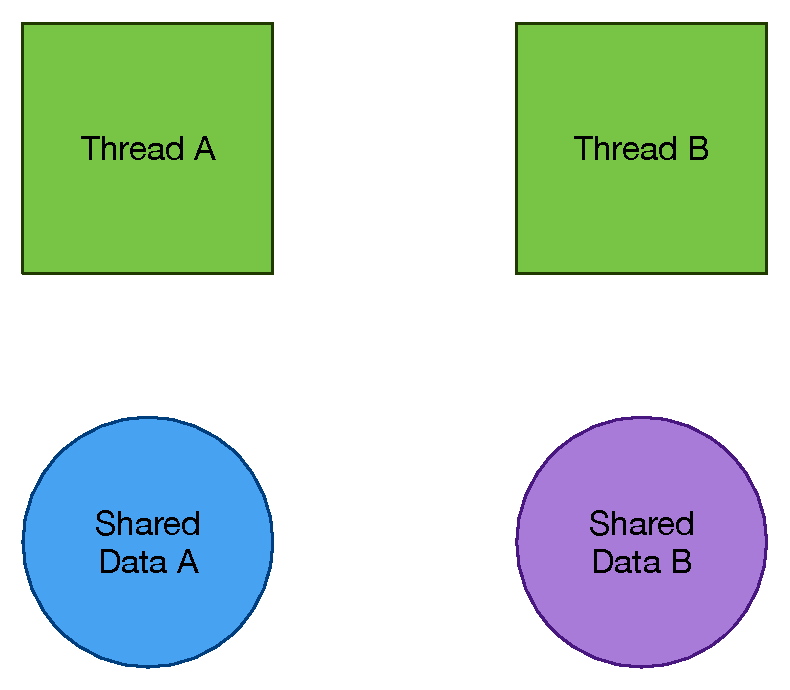
\includegraphics[width=0.7\textwidth]{../../figures/deadlock1.pdf}
\end{frame}

\begin{frame}
\centering
      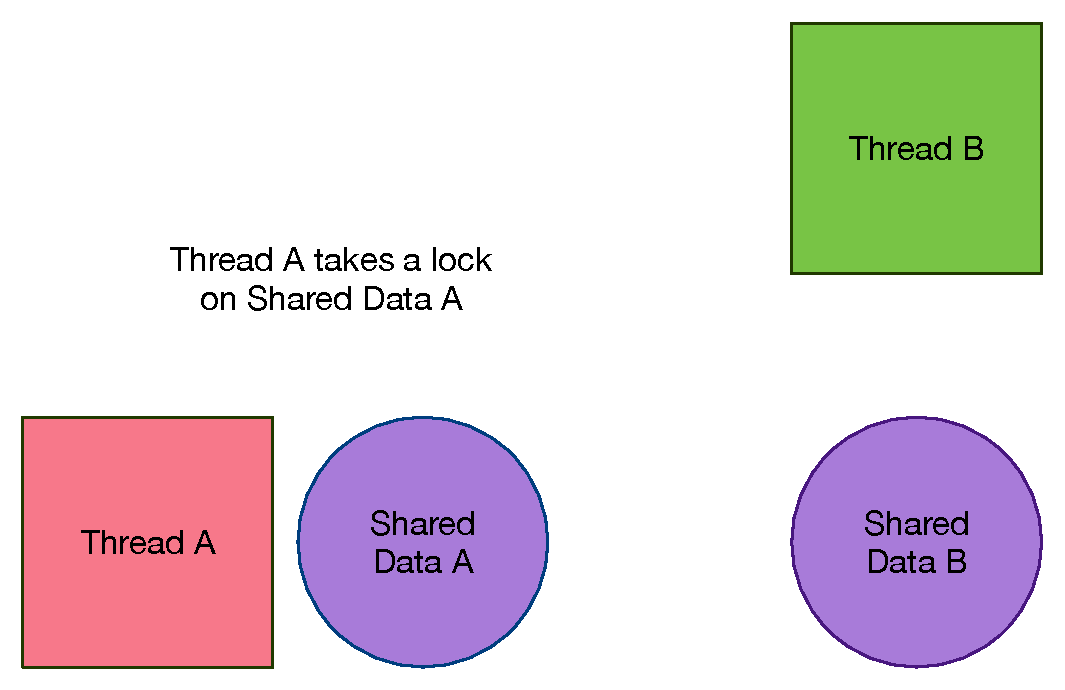
\includegraphics[width=0.8\textwidth]{../../figures/deadlock2.pdf}
\end{frame}

\begin{frame}
\centering
      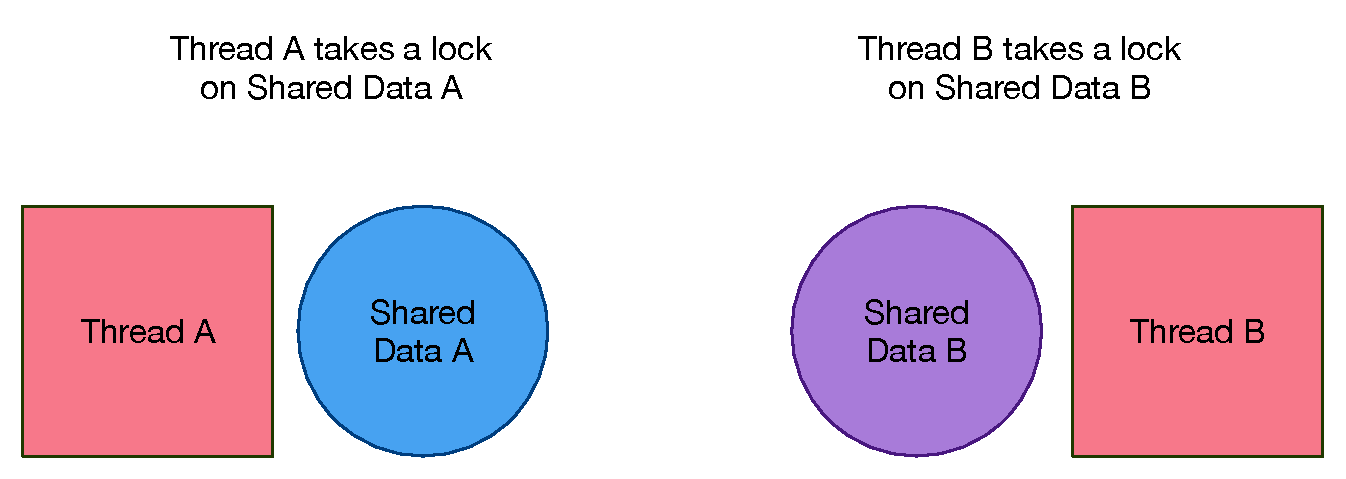
\includegraphics[width=\textwidth]{../../figures/deadlock3.pdf}
\end{frame}

\begin{frame}
\centering
      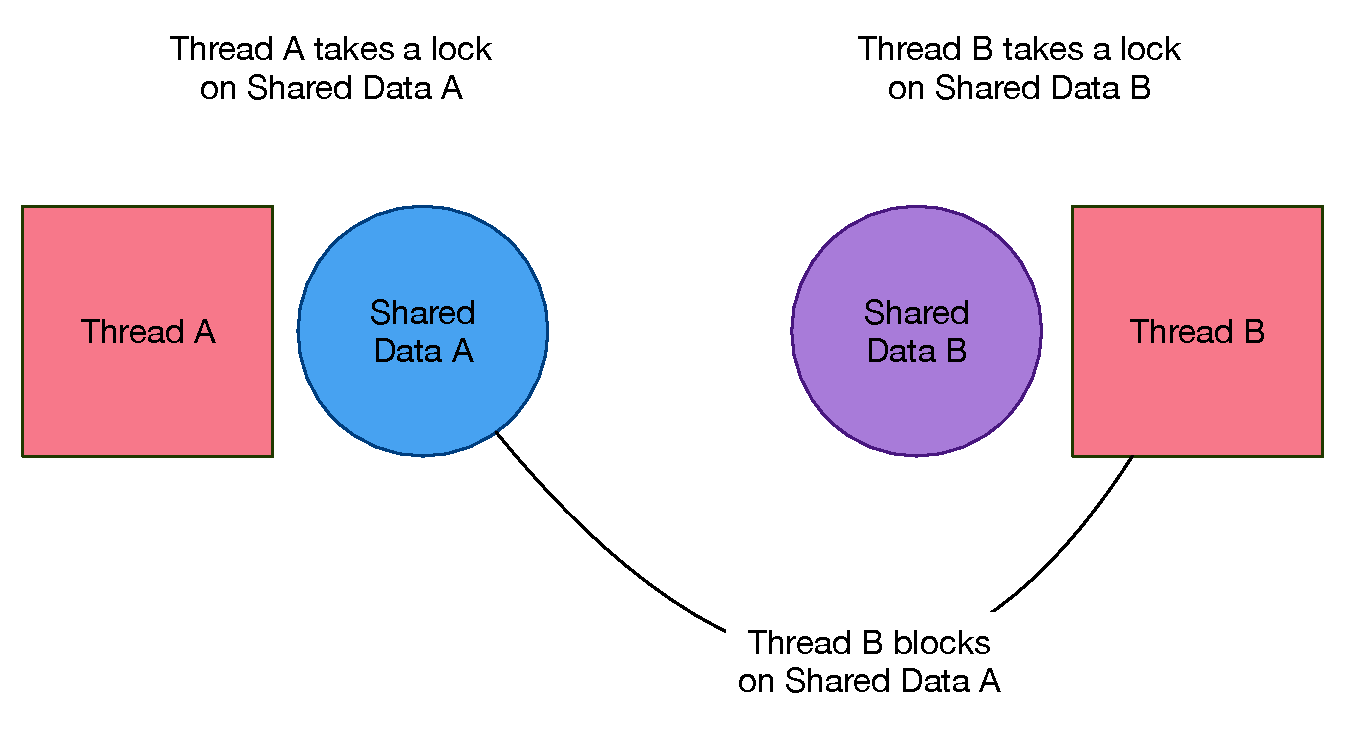
\includegraphics[width=\textwidth]{../../figures/deadlock4.pdf}
\end{frame}

\begin{frame}
\centering
      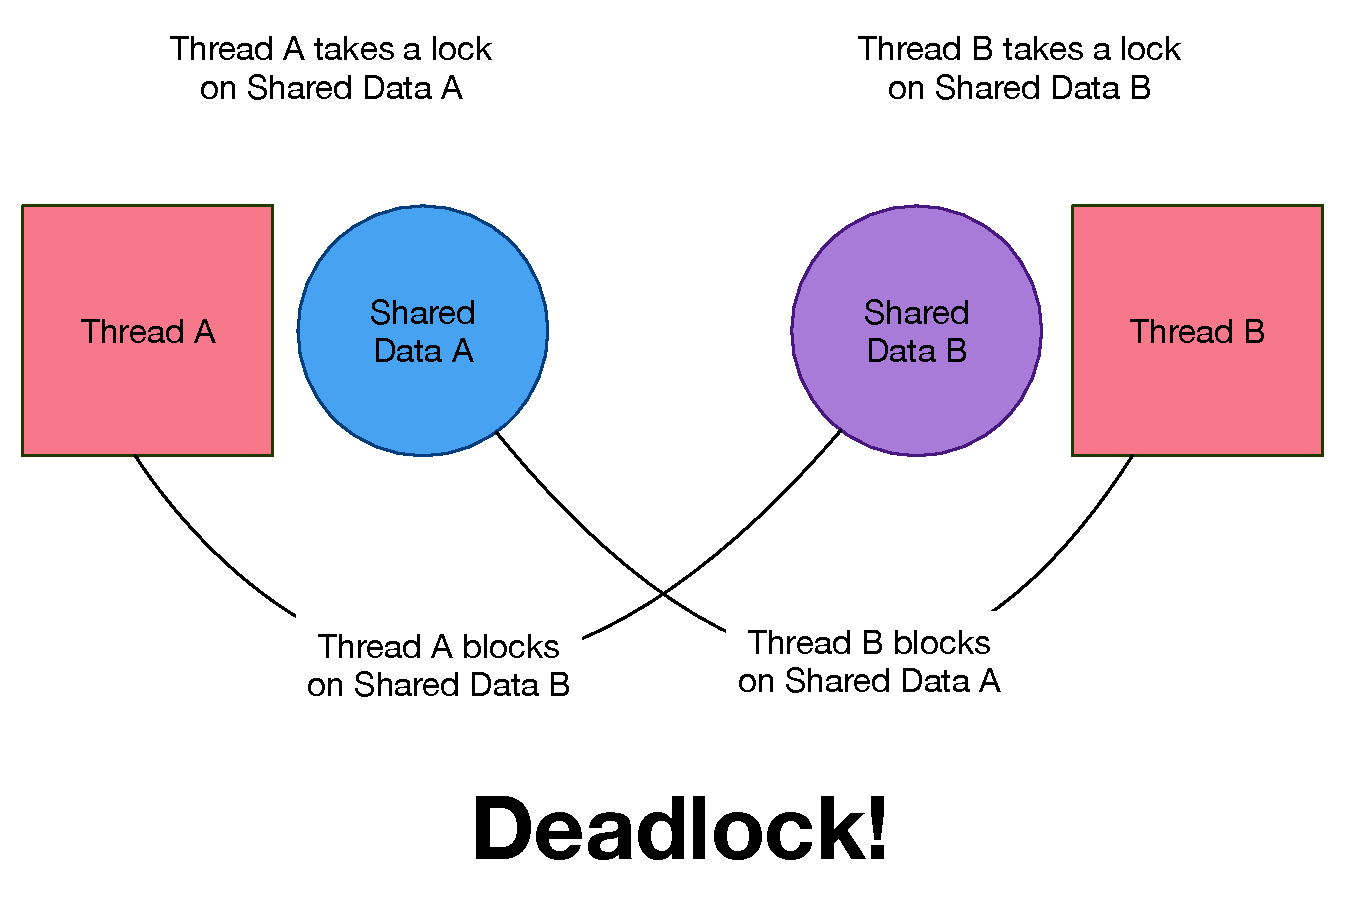
\includegraphics[width=\textwidth]{../../figures/deadlock5.pdf}
\end{frame}

\begin{frame}
\centering
      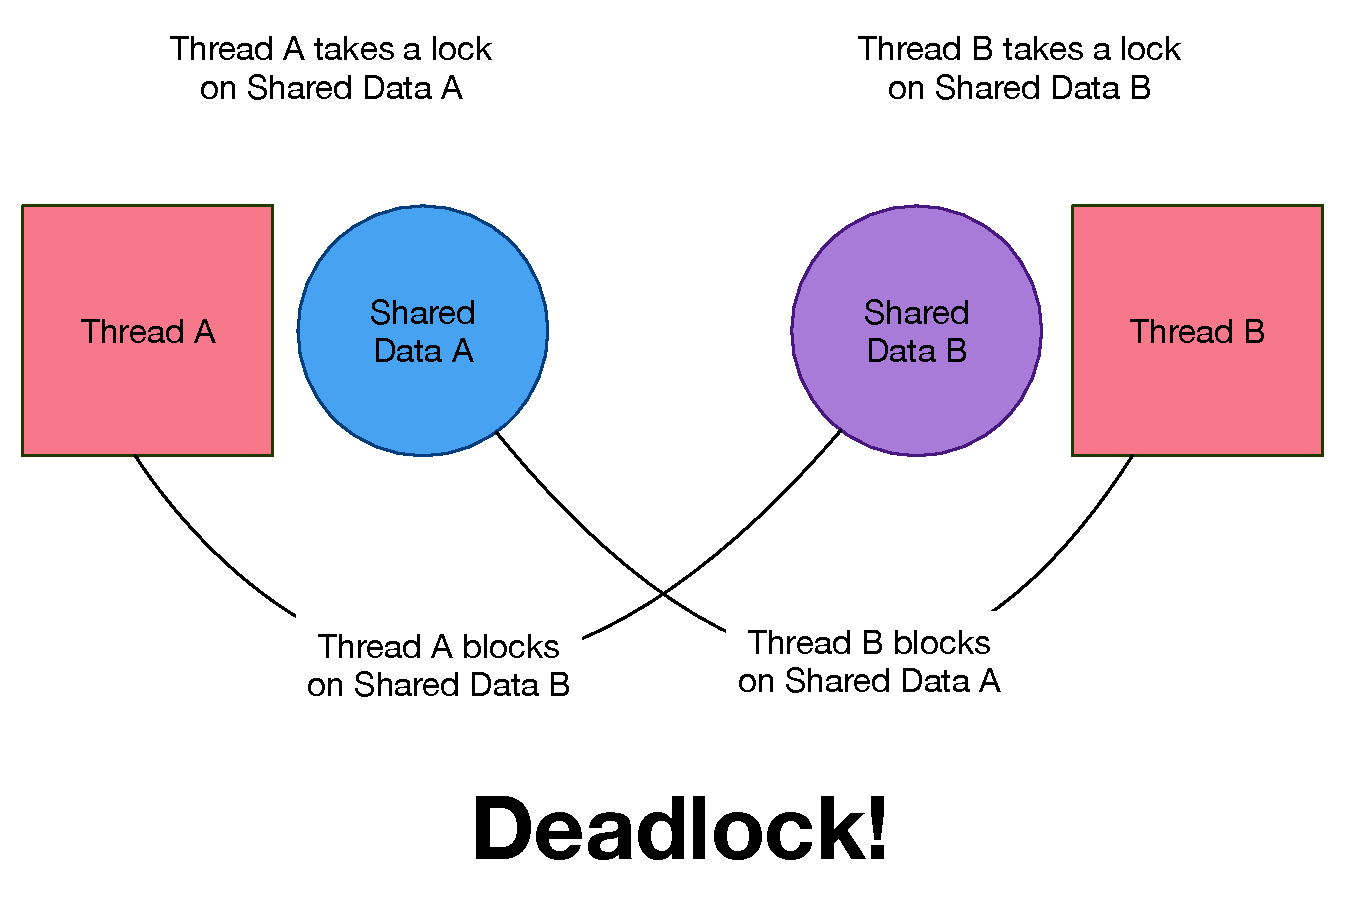
\includegraphics[width=\textwidth]{../../figures/deadlock6.pdf}
\end{frame}

\begin{frame}
  \frametitle{Locking Strategies}
  \begin{description}
  \item [Giant Lock] One big lock around the kernel
  \item [List Locks] Lock every list in the kernel.
  \item [Structure Locks] Lock individual structures
    \begin{itemize}
    \item Poorly chosen locking strategies impact performance
    \end{itemize}
  \end{description}
\end{frame}

\begin{frame}
  \frametitle{Types of Locks}
  \begin{description}
  \item[spin] Spin the CPU
  \item[mutex] Most basic lock
  \item[r/w lock] Reader/writer lock
  \item[sx lock] Shared/exclusive lock
  \end{description}
\end{frame}

\begin{frame}[fragile]
  \frametitle{Visualizing Locks with DTrace}
  \begin{itemize}
  \item The \verb|lockstat| provider
  \end{itemize}
\end{frame}

\begin{frame}
  \frametitle{The lockstat Provider}
  \begin{itemize}
  \item All lock types have similar probes
  \item 29 total probes in all
  \end{itemize}
  \begin{description}
  \item[acquire] Code grabbed the lock
  \item[block] Another thread was blocked
  \item[spin] Thread is spinning on the lock
  \item[release] Lock is released
  \end{description}
\end{frame}

\begin{frame}
  \frametitle{The lockstat Provider Arguments}
  \begin{description}
  \item[arg0] Address of lock object
  \item[arg1] Lock time or spin count
  \end{description}
\end{frame}

\begin{frame}[fragile]
  \frametitle{Who is locking?}
\begin{verbatim}
dtrace -n 'lockstat::: { @locks[execname] = count();} '
  nfsd                                                             16
  sudo                                                             35
  sendmail                                                         48
  fdc0                                                             56
  syncer                                                           68
  bufdaemon                                                       272
  sshd                                                            293
  kernel                                                          320
  vmdaemon                                                        670
...
\end{verbatim}
\end{frame}

\begin{frame}[fragile]
  \frametitle{Locking Review}
  \begin{itemize}
  \item Protection of shared resources
  \item Prevent incorrect updates
  \item Types of locks in FreeBSD
  \begin{description}
  \item[spin] Spin the CPU
  \item[mutex] Most basic lock
  \item[r/w lock] Reader/writer lock
  \item[sx lock] Shared/exclusive lock
  \end{description}
  \item The \verb|lockstat| provider
  \end{itemize}
  
\end{frame}

\section{The Illusion of Memory}
\label{sec:memory}

\begin{frame}
  \frametitle{Types of Memory}
  \begin{itemize}
  \item Stack
    \begin{itemize}
    \item Automatic variables
    \item Function call frames
    \end{itemize}
\pause
  \item Heap
    \begin{itemize}
    \item Pretty much everything else
    \end{itemize}
  \item Caches
    \begin{itemize}
    \item L1, L2, L3, etc.
    \end{itemize}
  \end{itemize}
\end{frame}

\begin{frame}
  \frametitle{The Illusion of Memory}
  \begin{itemize}
  \item How much memory can one process have?
  \item Early UNIX VM systems built on 32 bit hardware.
    \pause
    \begin{itemize}
    \item $4,294,967,296$ bytes
    \end{itemize}
    \pause
  \item Modern systems based on 64 bits.
    \begin{itemize}
    \item $18,446,744,073,709,551,615$ bytes
    \end{itemize}
  \item How does the OS manage this illusion?
  \end{itemize}
\end{frame}

\begin{frame}
  \frametitle{A brief history of memory}
  \begin{itemize}
  \item Delay Line
  \item Core
  \item Dynamic RAM
  \end{itemize}
\end{frame}

\begin{frame}
  \frametitle{Core}
  \begin{center}
    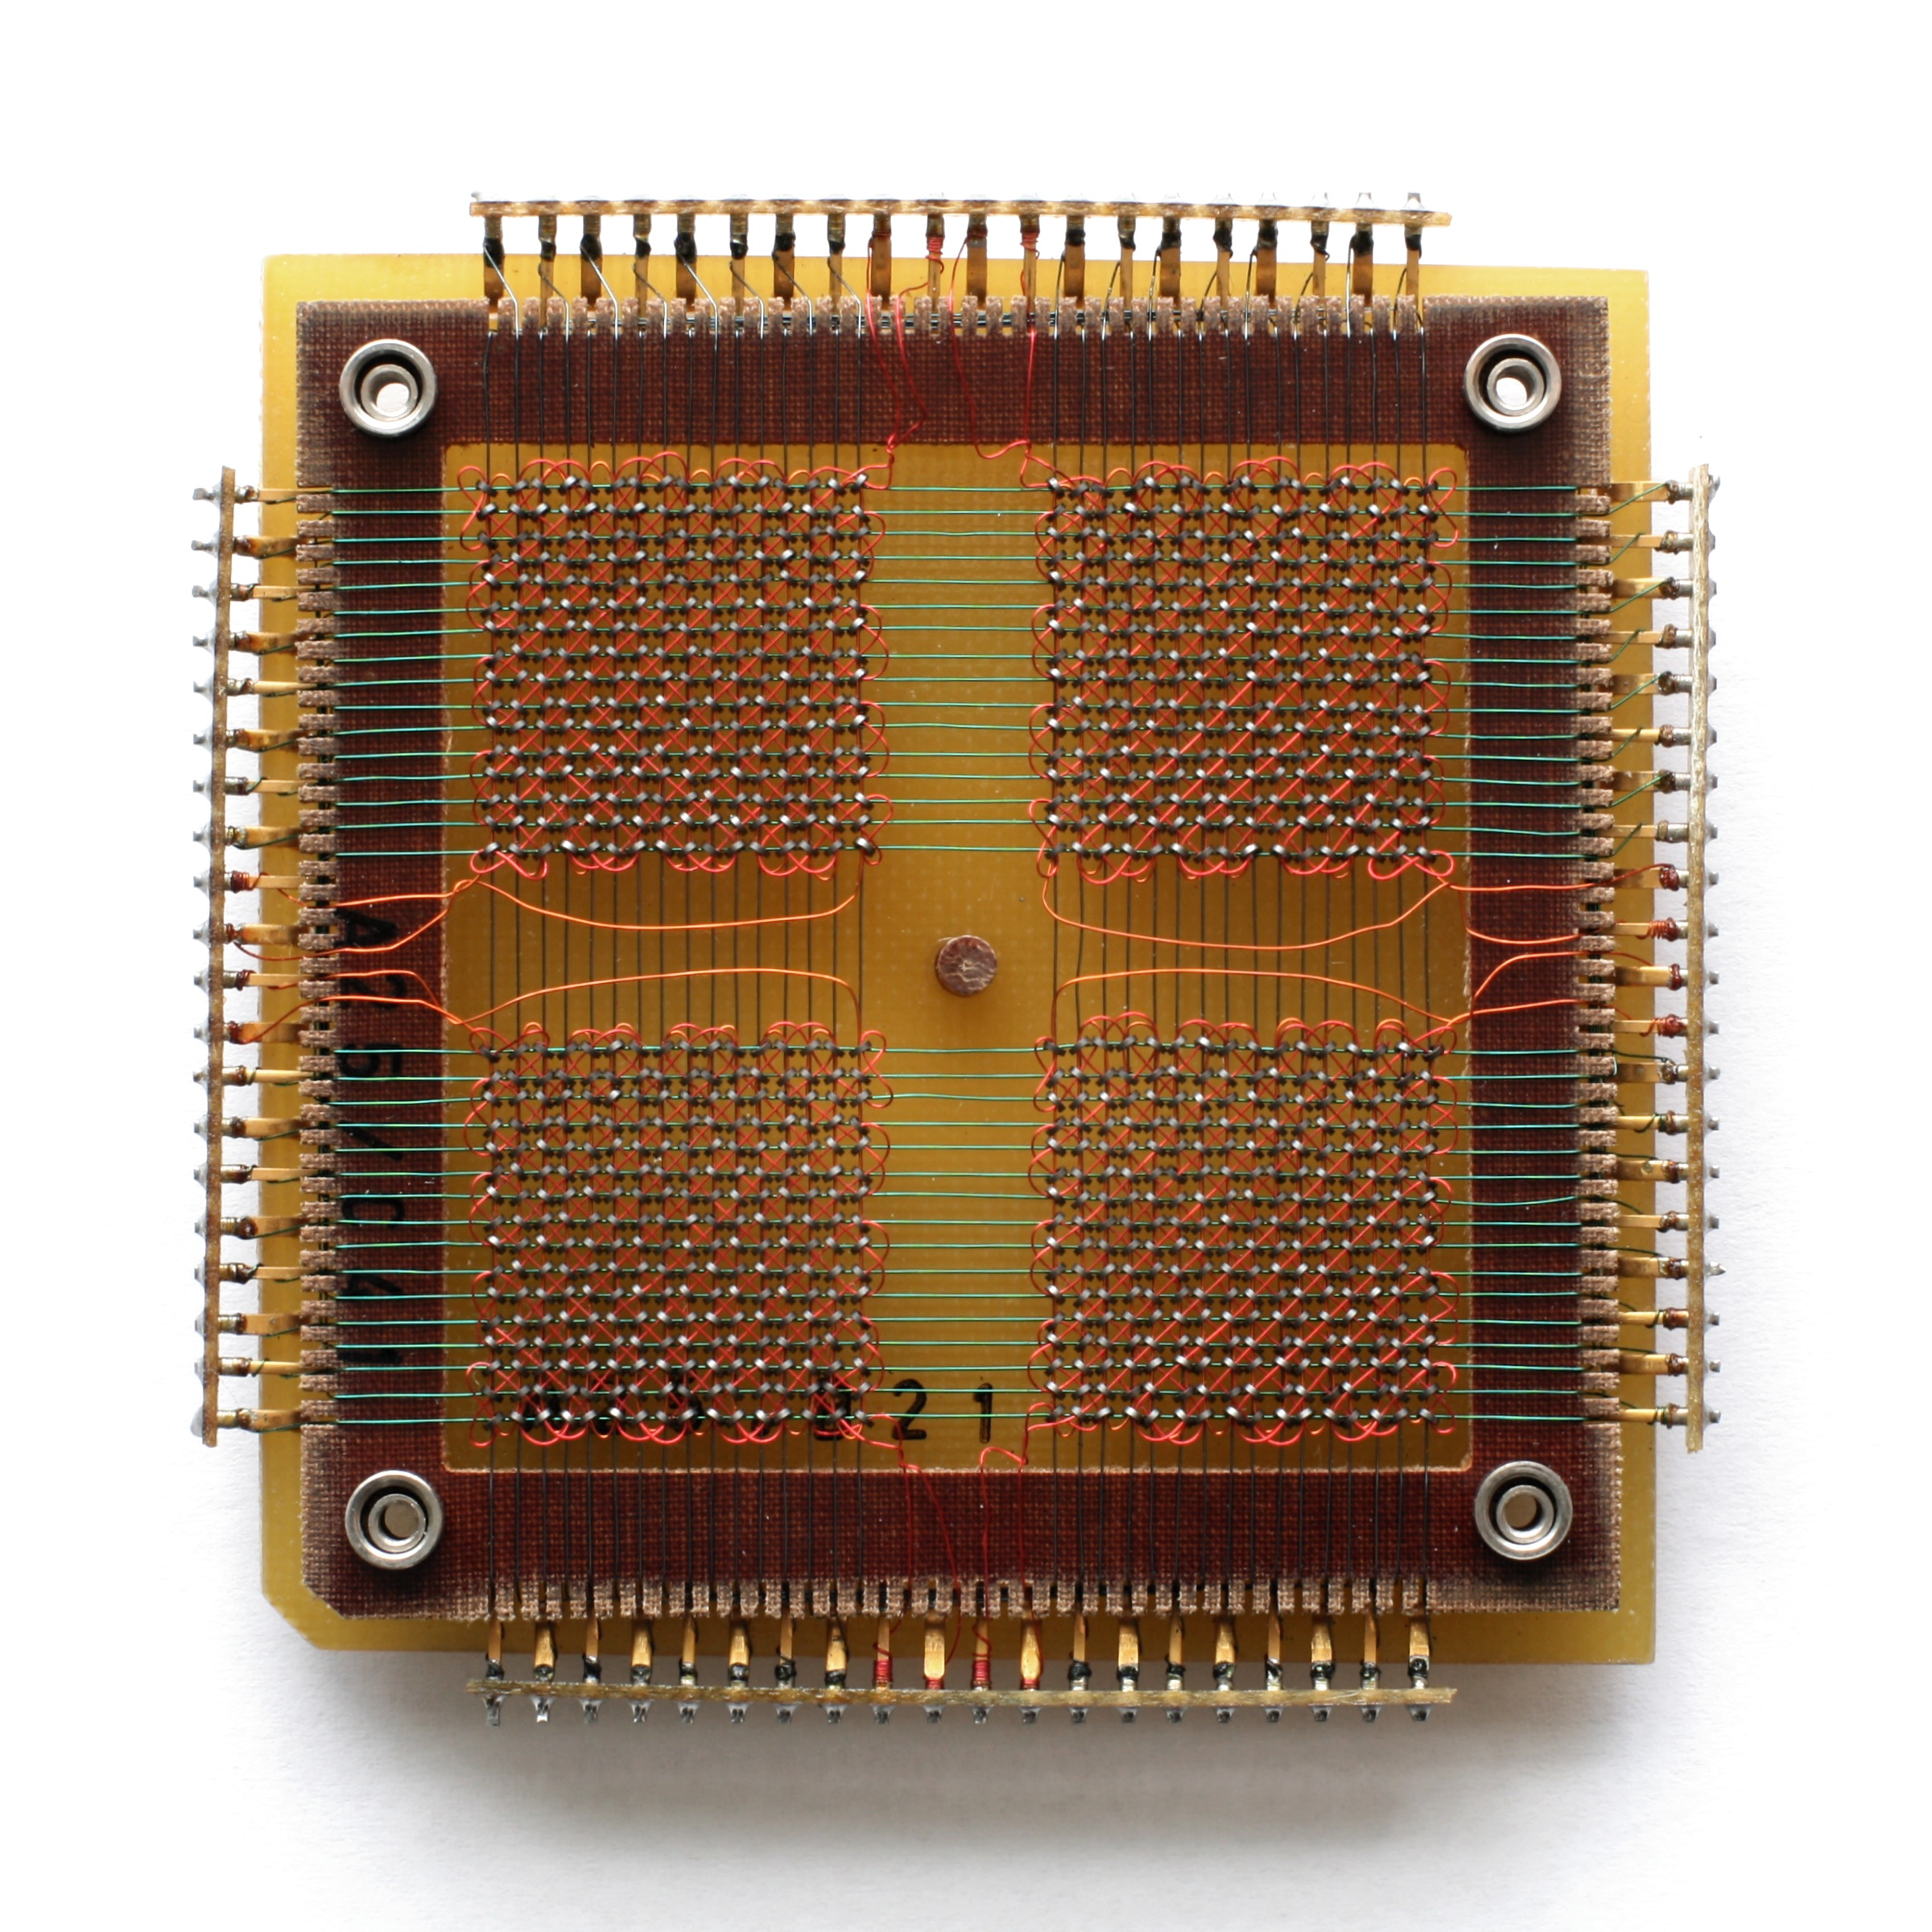
\includegraphics[width=0.8\textwidth]{../../figures/KL_CoreMemory.jpg}
  \end{center}
  
\end{frame}

\begin{frame}
  \frametitle{Core Close Up}
  \begin{center}
    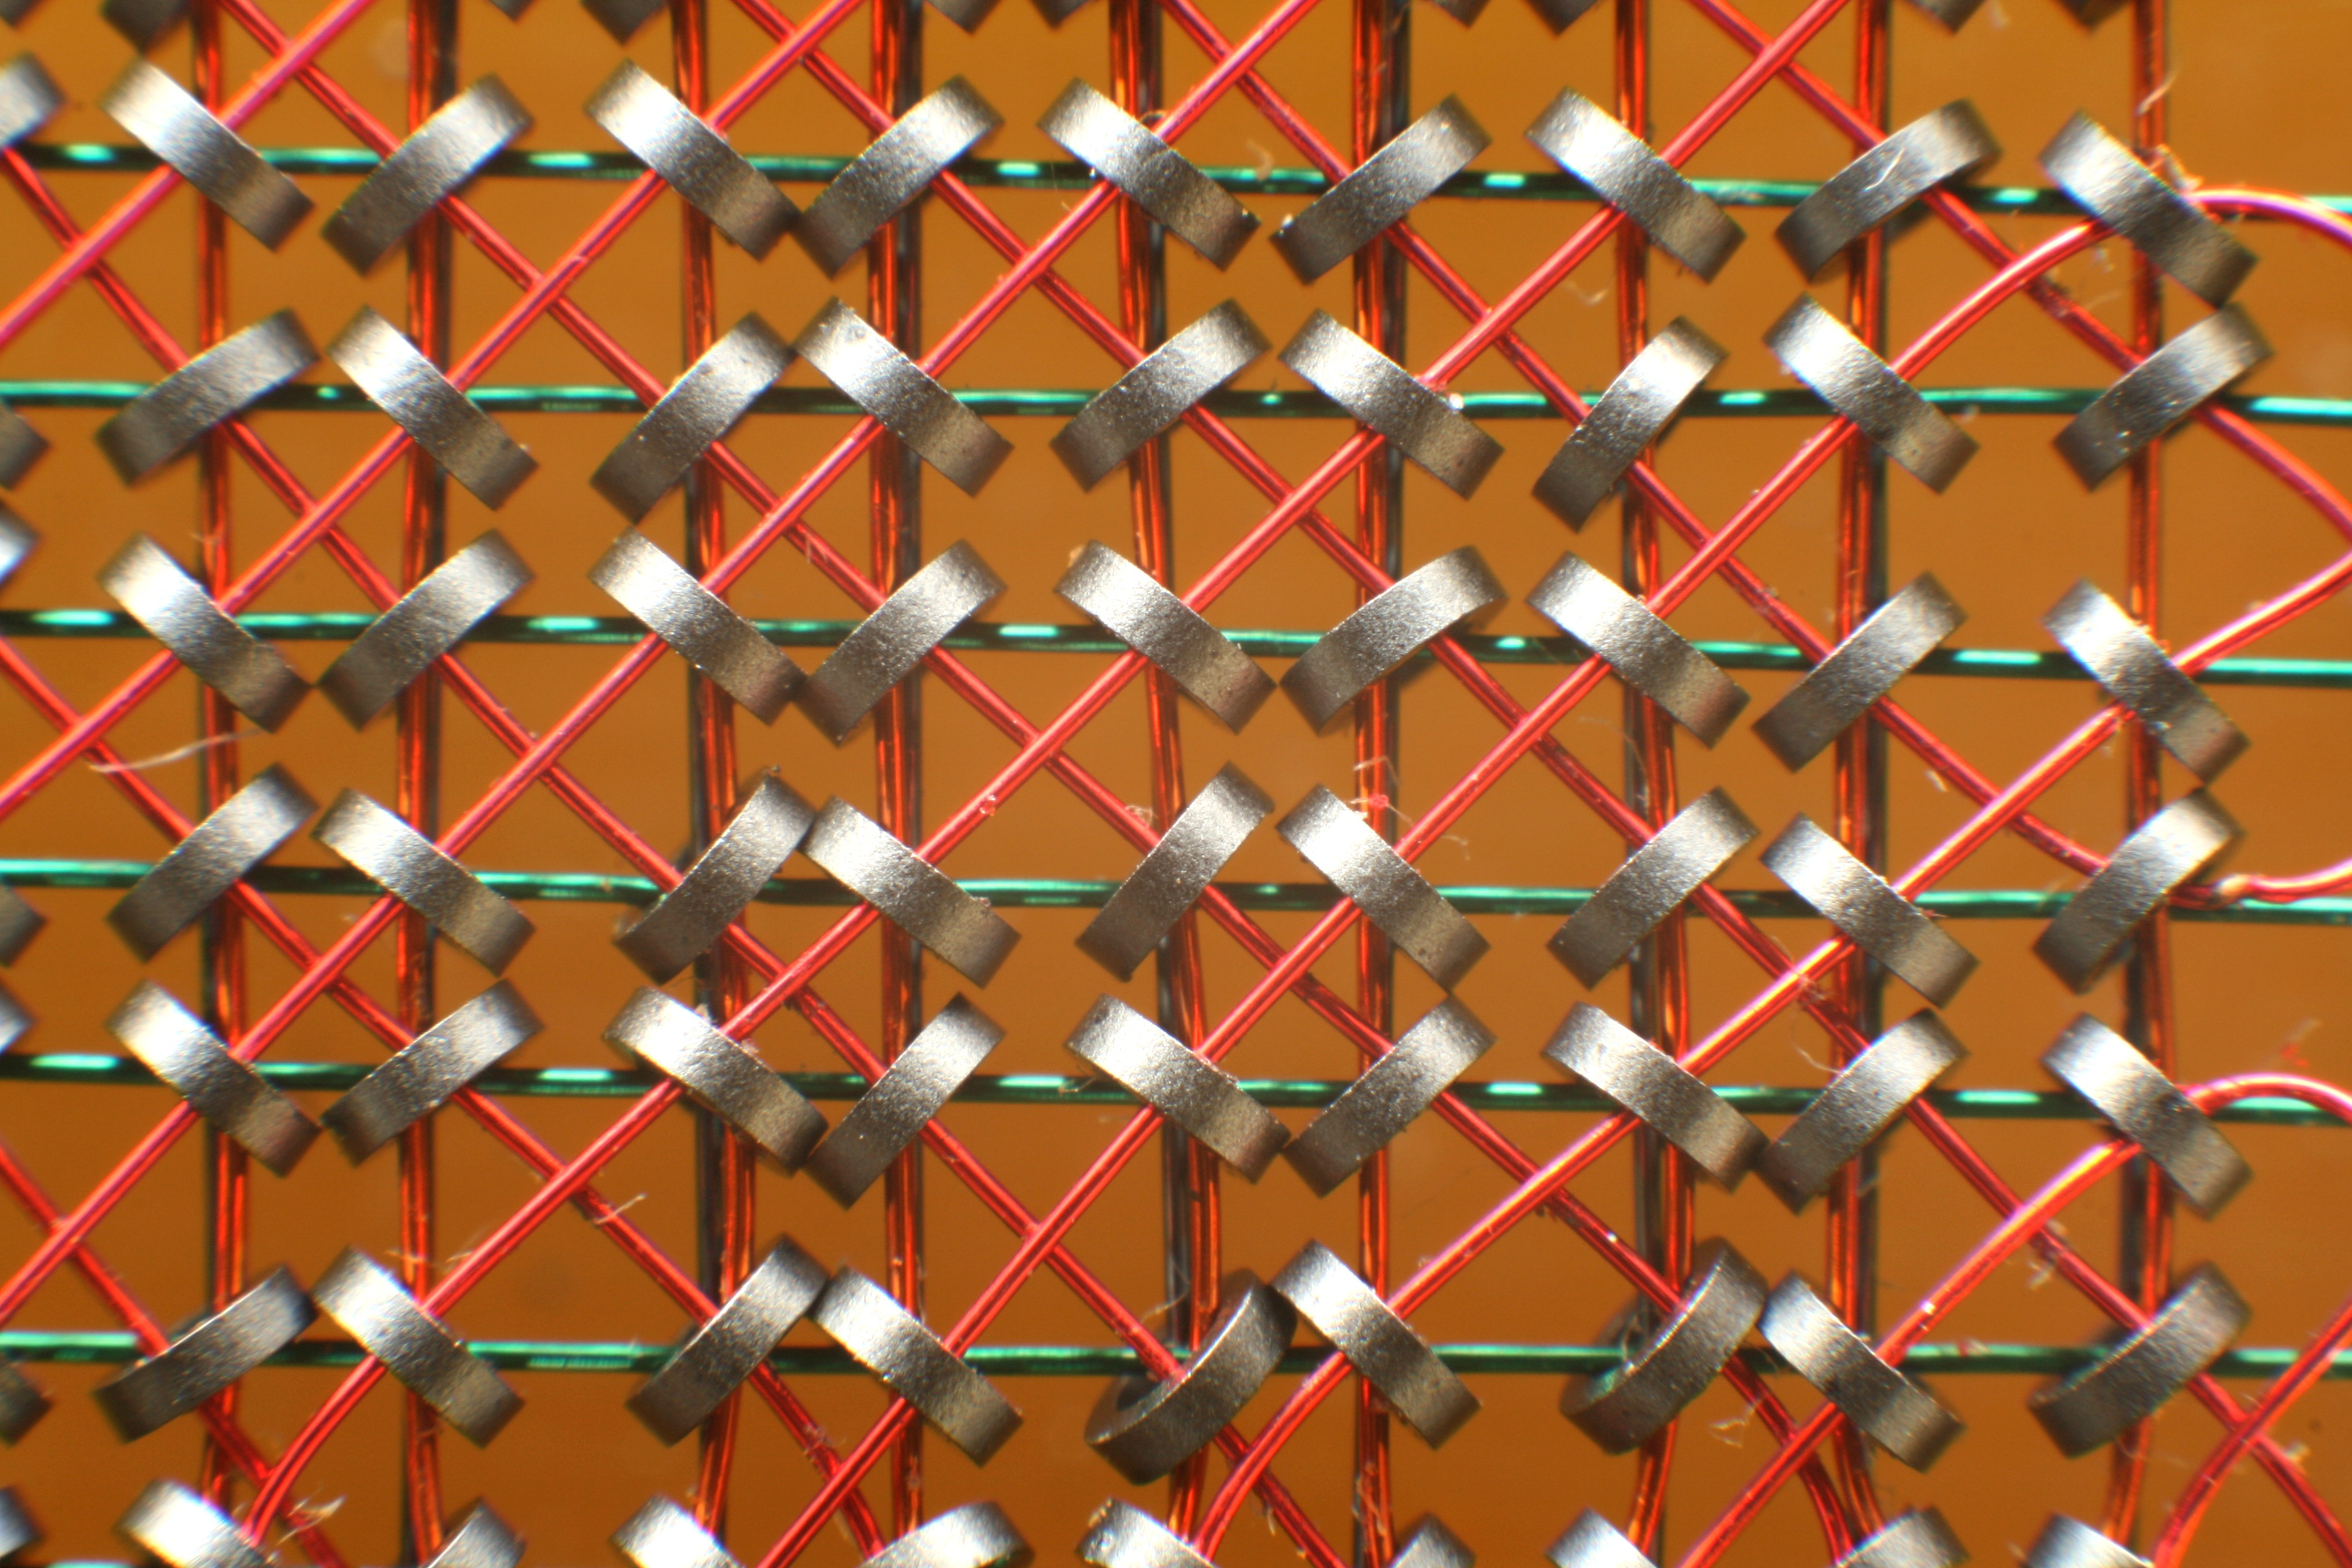
\includegraphics[width=0.8\textwidth]{../../figures/KL_Kernspeicher_Makro_1.jpg}
  \end{center}
\end{frame}

\begin{frame}
  \frametitle{A World Without Virtual Memory}
  \begin{itemize}
  \item Single Address Space Systems
  \item Embedded and Real Time Operating Systems (RTOS)
  \item These still exist
    \pause
    \begin{itemize}
    \item There are several on Mars
      \pause
    \item There are even more in automotive braking systems
    \end{itemize}
  \end{itemize}
\end{frame}

\begin{frame}
  \frametitle{But that's ridiculous!}
    \begin{center}
    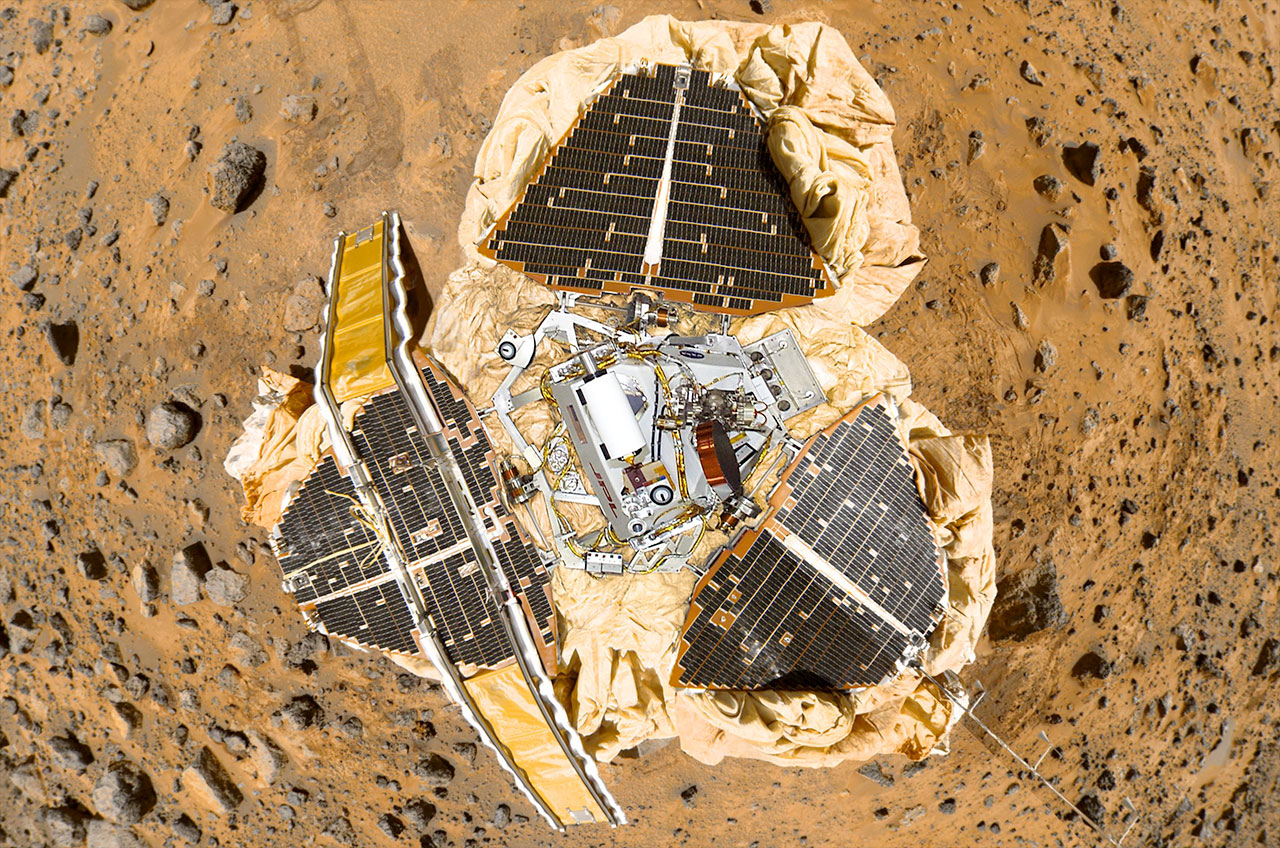
\includegraphics[width=0.8\textwidth]{../../figures/pathfinder.jpg}
  \end{center}

\end{frame}

\begin{frame}
  \frametitle{The Purpose of Virtual Memory}
  \begin{description}[labelwidth=\widthof{Simplification}]
  \item [Simplification] Programs (mostly) don't care about addresses.
  \item [Portability] No memory location is more special than any other.
  \item [Protection] All memory accesses go via the kernel.
  \end{description}
\end{frame}

\begin{frame}
  \frametitle{Two Programs in their Virtual Memory Spaces}

  \begin{center}
    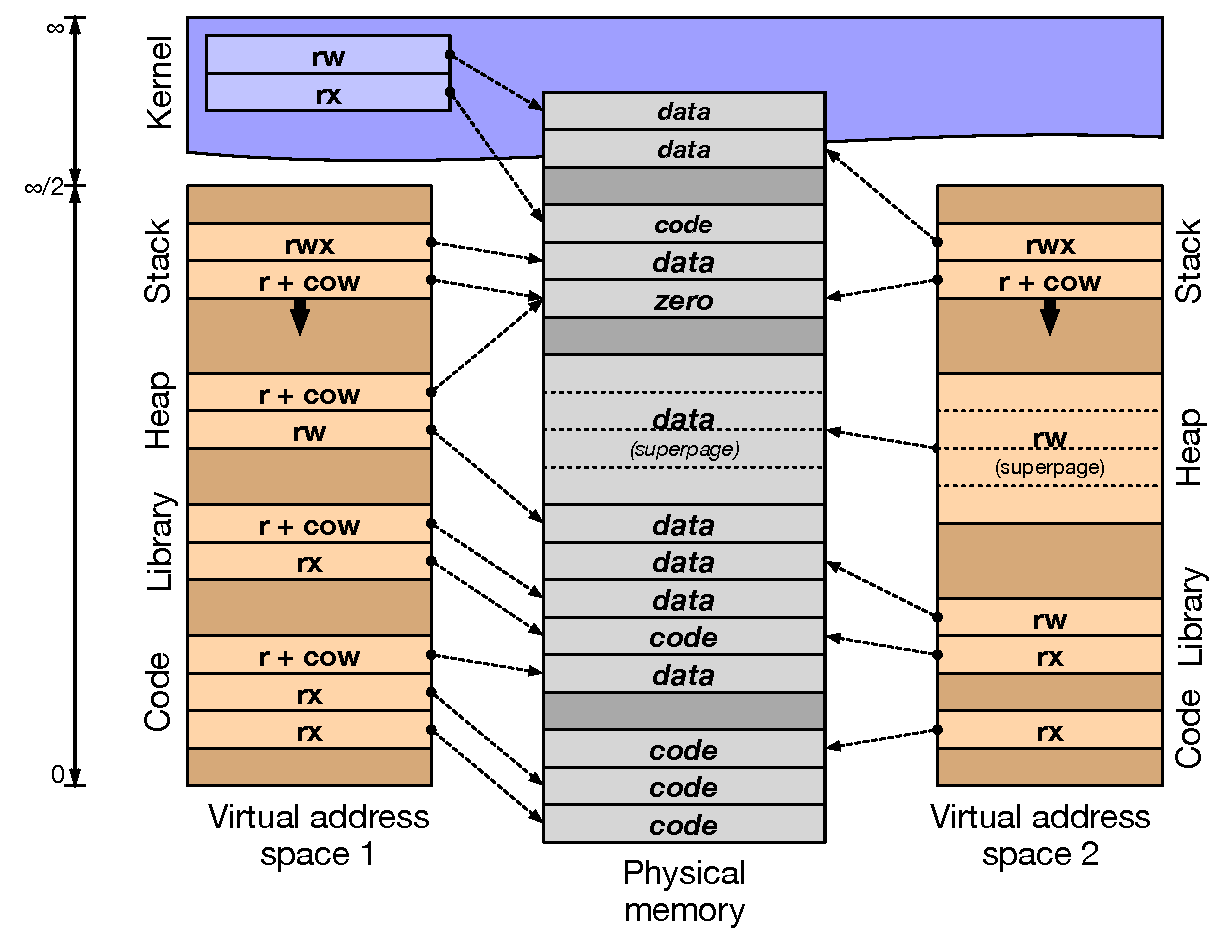
\includegraphics[width=0.8\textwidth]{../../figures/process-address-space.pdf}
  \end{center}
\end{frame}

\begin{frame}
  \frametitle{How does the VM trick work?}

  \begin{itemize}
  \item Virtual address spaces
    \begin{itemize}
    \item Isolation vs. sharing
    \item \textit{BSS}, \textit{Copy-on-Write}, \textit{Superpages}
    \end{itemize}
  \end{itemize}
\end{frame}

\begin{frame}
  \frametitle{How does the VM trick work?}

  \begin{itemize}

    \item Memory Management Unit (MMU)
    \begin{itemize}
      \item Transforms \textit{virtual addresses} into \textit{physical addresses}
      \item Memory is laid out in \textit{pages} (4K, 2M, 1G...)
      \item Control available only to the supervisor
      \item Software handles failures (e.g., permissions) via traps
    \end{itemize}
  \end{itemize}
\end{frame}

\begin{frame}
  \frametitle{How does the VM trick work?}

  \begin{itemize}

    \item Page tables
    \begin{itemize}
      \item SW-managed \textit{page tables} provide \textit{virtual-physical
	mappings}
      \item Access permissions, page attributes (e.g., caching)
      \item Various configurations + traps implement BSS, COW, sharing, ...
    \end{itemize}

  \end{itemize}
\end{frame}

\begin{frame}
  \frametitle{How does the VM trick work?}

  \begin{itemize}
    \item The Translation Look-aside Buffer (TLB)
    \begin{itemize}
      \item Hardware cache of entries -- avoid walking pagetables
      \item Content Addressable Memory (CAM); 48? 1024? entries
      \item TLB \textit{tags}: entries \textit{global} or for a specific process
      \item Software- vs. hardware-managed TLBs
    \end{itemize}

  \end{itemize}
\end{frame}

\begin{frame}
  \frametitle{Making Virtual Memory Work}
  \begin{itemize}
  \item Memory Management Unit (MMU)
  \item Page Tables
  \item Translation Look-aside Buffer (TLB)
  \end{itemize}
\end{frame}

\begin{frame}
  \frametitle{Observing Virtual Memory}
  
\end{frame}


\end{document}


%%% Local Variables:
%%% mode: latex
%%% TeX-master: "lecture2-processes.tex"
%%% End:
